
\documentclass[a4paper,10pt,oneside]{memoir}

%\usepackage{Packages}

\ProvidesPackage{Packages}

% \usepackage{floatrow}
\usepackage{a4wide}
\usepackage{amsmath}
\usepackage[italian]{babel}
\usepackage{fancyhdr}
\usepackage{gensymb}
\usepackage{graphicx,wrapfig}
\usepackage{grffile}
\usepackage{pifont}
\usepackage{float}

\usepackage{caption}
\captionsetup{format=plain, labelfont=bf, skip=0pt}

\usepackage{paralist}
\usepackage[usenames,dvipsnames]{color}
\usepackage{moreverb}
\usepackage{lscape}
%\usepackage[nottoc]{tocbibind}
\usepackage{verbatim}
\usepackage{datetime}
\usepackage{array}

\usepackage{color}
\definecolor{darkred}{rgb}{0.5,0,0}
\definecolor{darkgreen}{rgb}{0,0.5,0}
\definecolor{darkblue}{rgb}{0,0,0.5}
\definecolor{gray}{rgb}{0.35,0.35,0.35}

\usepackage[pagebackref=true,
            colorlinks=black,
            linkcolor=gray,
            bookmarks=true,
            filecolor=gray,
            urlcolor=gray,
            citecolor=gray
           ]{hyperref}

%\usepackage{titlesec}

%\titlespacing\section{0pt}{12pt plus 4pt minus 2pt}{0pt plus 2pt minus 2pt}
%\titlespacing\subsection{0pt}{12pt plus 4pt minus 2pt}{0pt plus 2pt minus 2pt}
%\titlespacing\subsubsection{0pt}{12pt plus 4pt minus 2pt}{0pt plus 2pt minus 2pt}

\usepackage{chngcntr}
\counterwithout{section}{chapter}

\usepackage{tocloft}

\usepackage{inputenc}
\usepackage{tikz}
\usepackage{anysize}
\usepackage{color} 
\marginsize{1.5cm}{1cm}{1cm}{2cm}
\usepackage[siunitx,european,americanresistors]{circuitikz}
\definecolor{logo}{HTML}{158388}
\definecolor{logo2}{HTML}{FFFFFF}
\definecolor{scritta}{HTML}{000000}

\def\sectionfont{\bfseries\LARGE}
\def\subsectionfont{\bfseries\Large}

%\renewcommand\cftsectionaftersnumb{\textbf}
\renewcommand{\cftsectionfont}{\normalfont\bfseries}% titles in bold

\usepackage{lipsum}

\setlength\cftsectionindent{0pt}
\setlength\cftsubsectionindent{15pt}
\setlength\cftsectionnumwidth{2em}
\setlength\cftsubsectionnumwidth{4em}

\renewcommand\cftbeforesectionskip{7pt plus 1pt}
\renewcommand\cftbeforesubsectionskip{4pt plus 1pt}

%\renewcommand\cftsecfont{\Large\bfseries}
%\renewcommand\cftsubsecfont{\large\bfseries}

%\renewcommand\cftsecpagefont{\large\bfseries}
%\renewcommand\cftsubsecpagefont{\large\bfseries}

%\renewcommand\cftsecafterpnum{\par\addvspace{15pt}}
%  \renewcommand\cftsubsecafterpnum{\par\addvspace{15pt}}



\usepackage{lineno}
\usepackage{longtable}
\usepackage[section]{placeins}
\usepackage{url}
\usepackage{makeidx}
\usepackage{hyperref}
\usepackage{subfig}

\usepackage{booktabs}
\usepackage{rotating}
\usepackage[absolute]{textpos}

\usepackage{listings}


\setlength{\parindent}{0.0in}
\setlength{\parskip}{0.1in}
\setlength{\marginparwidth}{2.3cm}

\newcommand\todo[1]{
  \-\marginpar[\raggedleft\footnotesize #1]
  {
    \raggedright\footnotesize #1
  }
}

\newcommand\ltodo[1]{
  \-\marginpar[\raggedleft\footnotesize ]
  {
    \raggedright\footnotesize
  }
}

%\docdate
%\newcommand{\docdate}{\today}

%\newcommand{\clearemptydoublepage}{
%    \newpage{\pagestyle{empty}
%    \cleardoublepage}
%}

\fancypagestyle{plain}{
\fancyhf{}
\fancyfoot[LO,RE]{\doctitle}
\fancyfoot[RO, LE]{\thepage}
\renewcommand{\headrulewidth}{0pt}
\renewcommand{\footrulewidth}{0.4pt}}

\pagestyle{plain}

\modulolinenumbers[5]

\newcommand{\tick}{\textcolor{darkgreen}{\ding{51}}}
\newcommand{\cross}{\textcolor{darkred}{\ding{55}}}
\usepackage[framed,numbered,autolinebreaks,useliterate]{Listings}


\addto\captionsbritish{\renewcommand{\contentsname}{Indice}}

%\linenumbers

\newcommand{\researchgroup}{LABORATORIO DI FISICA I}

\newcommand{\doctitle}{Laboratorio di Fisica - Esperienza di Elettrostatica}



\begin{document}
\counterwithout{figure}{chapter}
\counterwithout{figure}{section}
% SECTIONS
\makeatletter
\setsecheadstyle{\tikz{
\fill[logo](1,-1.85) rectangle (14,-2);
\node[inner sep=0pt,outer sep=0pt,text=white,scale=1.5,font=\sectionfont]  at (.5,-1.35) {\color{scritta}\Large\thesection};

    
}\vskip-9ex\hskip5em\sectionfont\color{scritta}}
% SUBSECTIONS
\setsubsecheadstyle{\tikz{
\fill[logo](1.5,-3.90) rectangle (8,-4);
\node[inner sep=0pt,outer sep=0pt,text=logo,scale=1,font=\sectionfont]  at (.5,-3.43)  {\color{scritta}\quad\thesubsection};
\node[inner sep=0pt,outer sep=0pt,text=logo2,scale=1,font=\sectionfont]  at (1.6,-3.5){$\gg$};
}\vskip-8ex\hskip5em\subsectionfont\color{scritta}
}
\setcounter{tocdepth}{2}
\setcounter{secnumdepth}{2}% to number subsubsections

\def\@seccntformat#1{\hskip0em}
\makeatother

\setbeforesecskip{\onelineskip}
\setaftersecskip{2\onelineskip}



\setbeforesubsecskip{-1\onelineskip}
\setaftersubsecskip{2\onelineskip}


\setbeforesubsubsecskip{-1\onelineskip}
\setaftersubsubsecskip{3\onelineskip}



\pagenumbering{gobble}
\begin{center}
\vspace*{5.8cm}

\setlength{\TPHorizModule}{1mm}
\setlength{\TPVertModule}{\TPHorizModule}

\newlength{\backupparindent}
\setlength{\backupparindent}{\parindent}
\setlength{\parindent}{0mm}

\begin{textblock}{155}(30,20)
    \vspace*{1mm}
    \huge
    \textbf{Esperienza di Elettrostatica\\}
    \LARGE
    \vspace*{5mm}

    {Studio sperimentale dei fenomeni elettrostatici}
    \par
    \vspace*{15mm}
    \Large
    \begin{textblock}{155}(30,60)
    \begin{flushleft}
        \Large
             \textbf{Componenti:} Vittorio Strano, Arianna Genuardi, Florinda Tesi, Antonio Riolo, Matteo Romano
    \end{flushleft}
    \end{textblock}
\end{textblock}

\setlength{\parindent}{\backupparindent}
\end{center}

\tableofcontents*

\newpage
\normalsize
\pagenumbering{arabic}

%qui vanno messe le sezioni, nella forma

\section{Introduzione}
{\fontsize{12}{14}\selectfont
Con questo esperimento si vogliono analizzare le caratteristiche di un condensatore a facce piane e parallele, in particolare come la capacità $C$ dipenda dalla quantità di carica $Q$ e dalla differenza di potenziale $V$ seguendo l'\autoref{eq:C(Q,V)}

\begin{equation} \label{eq:C(Q,V)}
    C = \frac{Q}{V}
\end{equation}

oltre che dalla costante dielettrica del mezzo tra le armature $\varepsilon$ e dalla distanza tra le facce $d$ che, in approssimazione $d \ll \sqrt{A}$, segue l'equazione l'\autoref{eq:capacitacondensatore},

\begin{equation} \label{eq:capacitacondensatore}
    C = \varepsilon \frac{A}{d}
\end{equation}

dove $A$ indica la superficie delle armature.

Per stimare la capacità dell'\emph{ice pail}, approssimata a quella di un condensatore cilindrico, è stata utilizzata l'\autoref{eq:capacitagabbia}, 

\begin{equation} \label{eq:capacitagabbia}
    C = \dfrac{2 \pi \varepsilon L}{\ln{\left(\dfrac{D_2}{D_1}\right)}}
\end{equation}

dove $L =$ altezza, $D_1 =$ diametro interno e $D_2 =$ diametro esterno dell'\emph{ice pail}.
\par}
 

\section{Metodi sperimentali}
\subsection{Strumentazione}
{\fontsize{11}{14}\selectfont 
Gli strumenti utilizzati in questa esperienza sono:
\begin{enumerate}
    \item \textbf{Calibro ventesimale} con un errore di $0.01 cm$
    \item \textbf{Righello} con un errore di $0.05 cm$
    \item \textbf{Condensatore a facce piane ES-9079} con facce circolari di diametro $(17.8 \pm 0.1) cm$ e superficie $A = (249 \pm 3) cm^2$. La facce sono mobili e poste su un binario dotato di riga graduata con errore $0.5 mm$ e distanza massima $d = 10 cm$. Prima di ogni parte dell'esperimento è stato necessario assicurarsi che la armature fossero parallele regolandone l'inclinazione
    \item \textbf{Elettrometro ES-9078A} con errore di precisione dell'$1\%$ sul f.s. + 1 digit, dotato delle seguenti scale: $(1, 3, 10, 30, 100)V$ e costituito da una capacità interna del valore tabulato $C_e = 28 \pm 3 pF$
    \item \textbf{Generatore di tensione ES-9077} con d.d.p. fissate a $30 V$ $\pm 5\%$ e $1$, $2$ e $3 kV$ $\pm 10\%$
    \item \textbf{Sfera conduttrice ES-9059}
    \item \textbf{\emph{Proof plane}} di diametro $(3.20 \pm 0.01) cm$
    \item \textbf{\emph{Ice pail}} la cui capacità è stata calcolata seguendo l'\autoref{eq:capacitagabbia} dopo aver misurato con il calibro $L = (15.54 \pm 0.01) cm$, $D_1 = (9.94 \pm 0.01) cm$ e $D_2 = (14.75 \pm 0.17) cm$, quest'ultima non essendo uniforme è stata calcolata come media e semi-dispersione del massimo $D_{2 \; max} = 14.92 cm$ e del minimo $D_{2 \; min} = 14.58 cm$
    \item \textbf{Cavi} a bassa capacità
    \item \textbf{Tavola di legno} di spessore $(1.04 \pm 0.01)cm$% di superficie sufficiente a coprire l'armatura del condensatore
\end{enumerate}

\par} 
\subsection{Procedimento Parte I}
{\fontsize{12}{14}\selectfont 

Il circuito utilizzato è costituito dall'elettrometro collegato al condensatore e dalla sfera conduttrice connessa a una delle uscite del generatore, posizionata ad almeno $50cm$ dal condensatore in modo che non sia presente una carica aggiuntiva dovuta ad un processo di induzione. 
\\
Il sistema formato dall'elettrometro e dal condensatore può essere schematizzato nel modo seguente:

\begin{figure}[H]
  \begin{minipage}[c]{0.4\textwidth}
    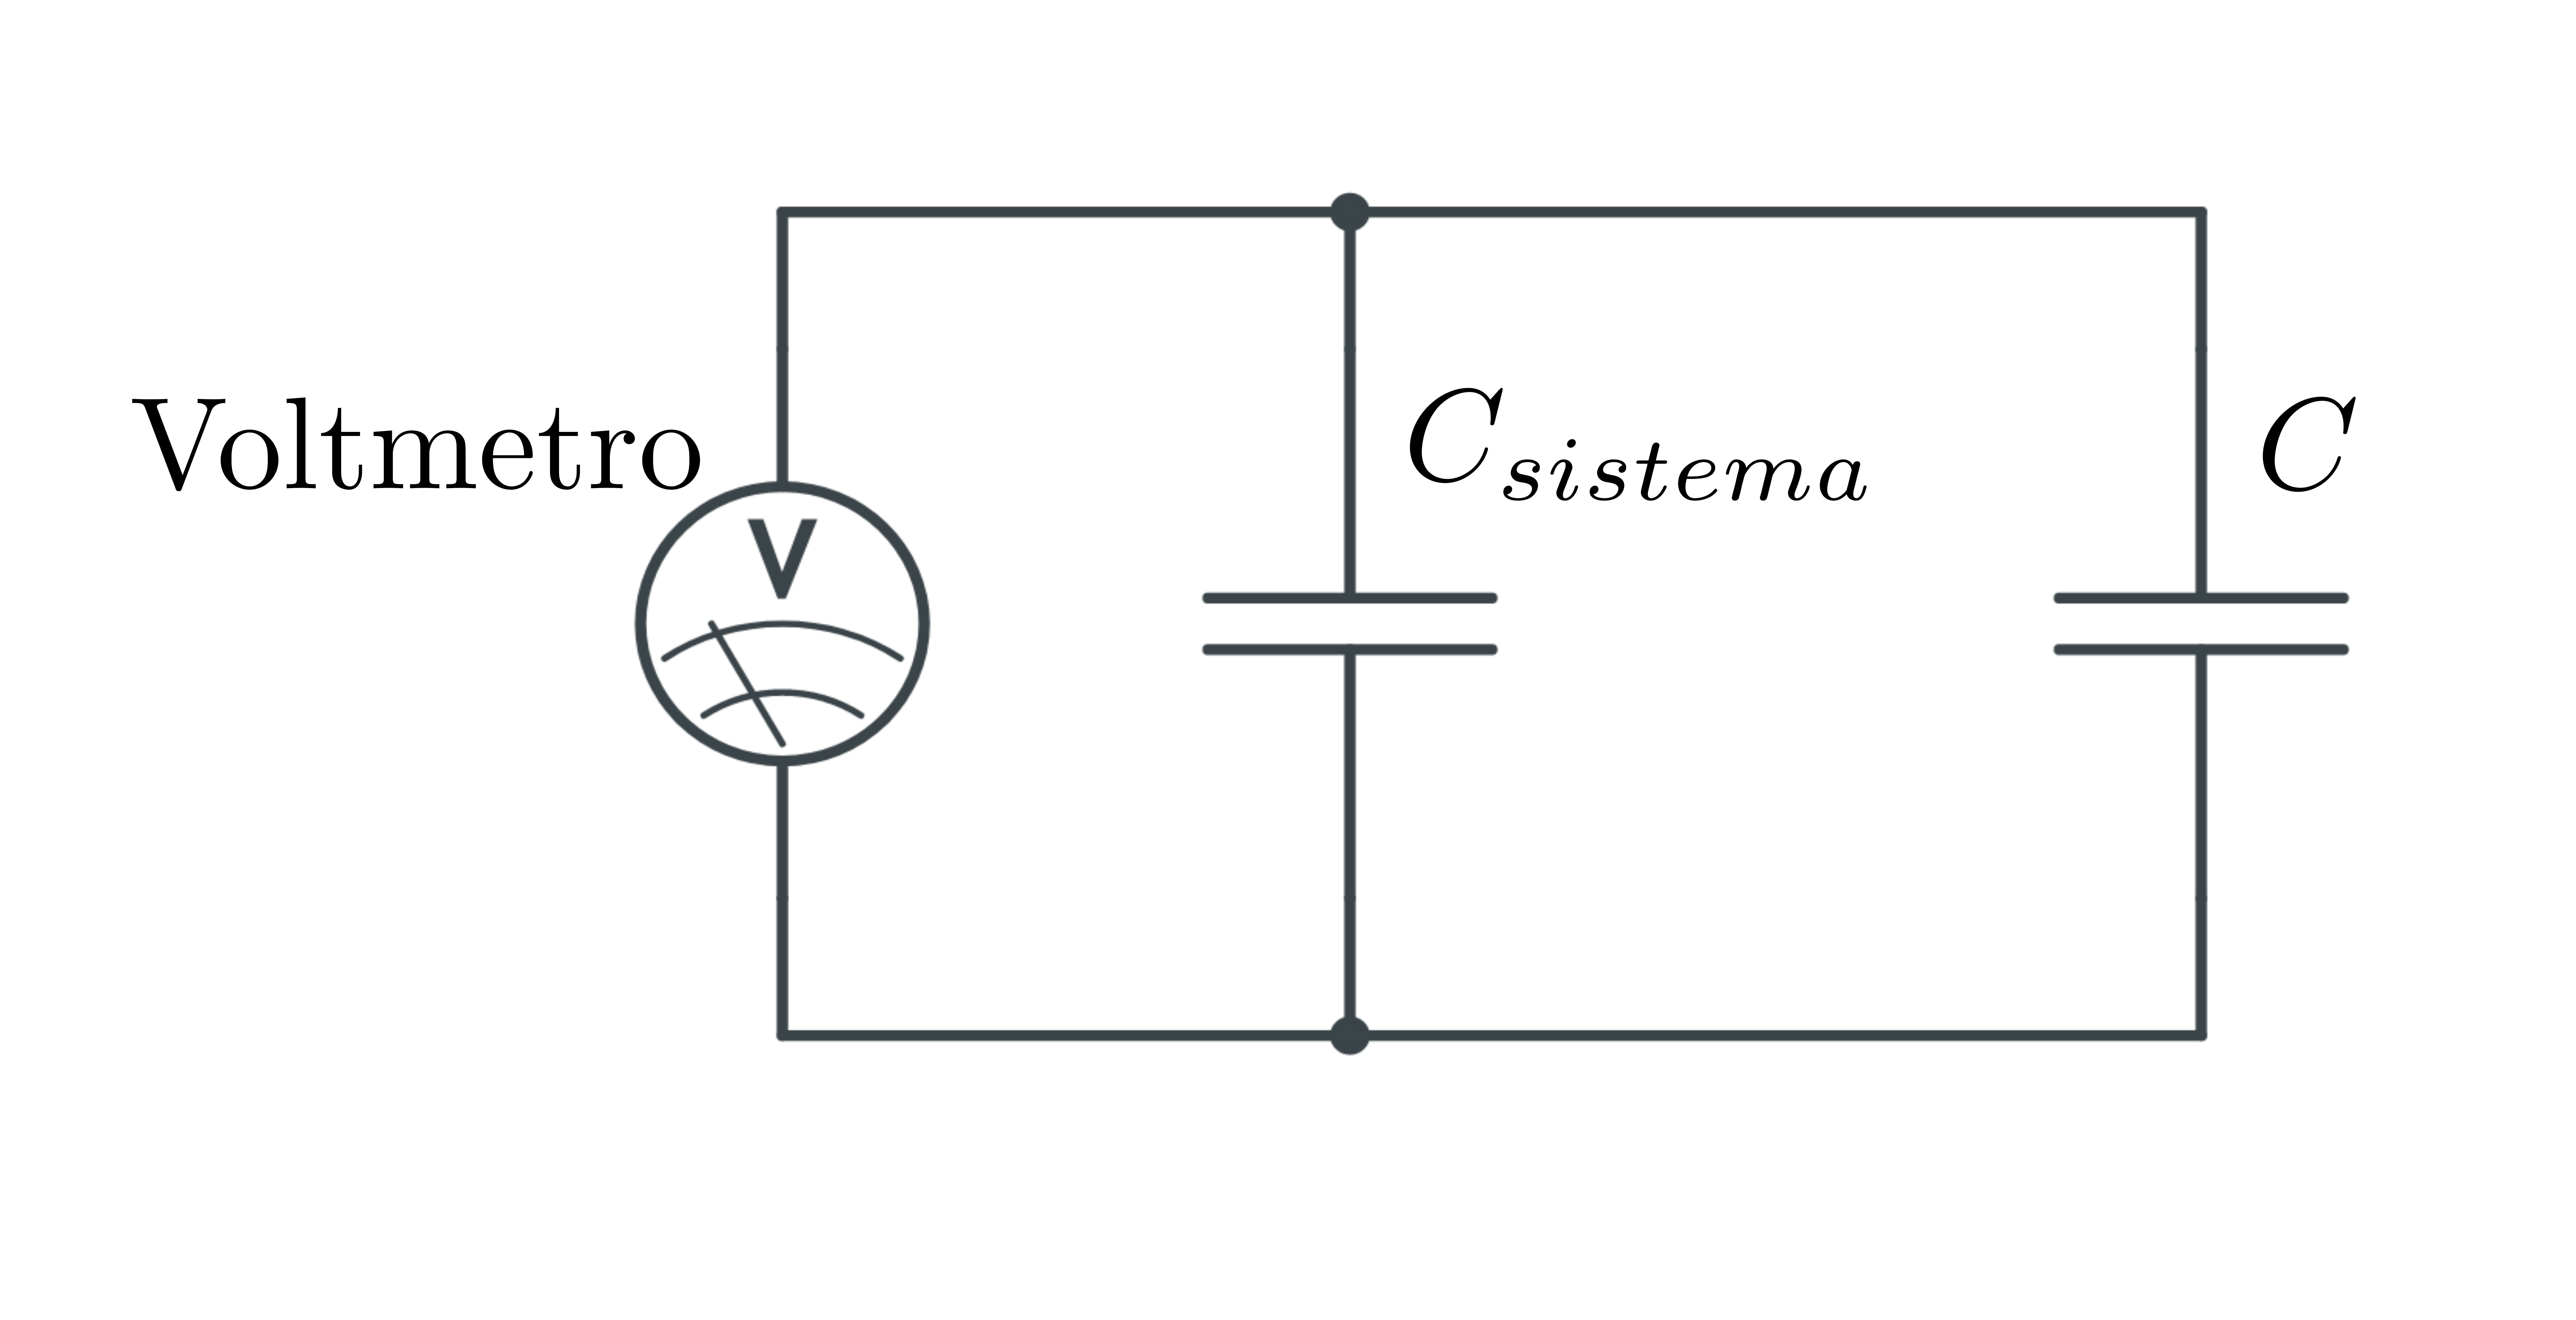
\includegraphics[width=8cm]{Figures/SchemaCircuitale3.png}
  \end{minipage}\hfill
  \begin{minipage}[c]{0.55\textwidth}
    \caption{
       Il circuito in figura mostra $C_{sistema}$ = capacità del sistema formato dall'elettrometro insieme ai suoi cavi, in parallelo con il condensatore $C$.
    } \label{fig:schemacircuitale}
  \end{minipage}
\end{figure}


Con la \emph{proof plane} è stata toccata prima la sfera e poi il condensatore per trasferire la carica, facendo in modo che le superfici fossero tangenti e che il contatto avvenisse sempre nello stesso punto. Dopo aver toccato il condensatore è stata rimossa la carica residua dalla \emph{proof plane} mettendola a contatto con la massa.

A diverse distanze tra le facce delle armature è stata trasferita la carica con $5$ tocchi ed è stata rilevata la misura della tensione con l'elettrometro.

Sono stati scelti 5 tocchi per sfruttare al meglio il fondoscala dell'elettrometro ed ottenere il miglior rapporto segnale/rumore.


Questo procedimento è stato ripetuto per sei diversi set di misura facendo variare al massimo un parametro alla volta:

\begin{enumerate}
    \item \textbf{Set$_1$} 3000V - 5 tocchi
    \item \textbf{Set$_2$} 3000V - 5 tocchi
    \item \textbf{Set$_3$} 3000V - 5 tocchi
    \item \textbf{Set$_4$} 2000V - 5 tocchi
    \item \textbf{Set$_5$} 3000V - 5 tocchi - 3s delay prima di trasferire la carica al condensatore
    \item \textbf{Set$_6$} 3000V - sfera a circa $12cm$ da un'armatura
\end{enumerate}

Sono state poi plottate le tensioni in funzione delle distanze ed è stato fatto un fit, prendendo in considerazione solo i punti fino a $d = 2 cm$, ovvero in approssimazione $d \ll \sqrt{A} = 15.8 cm$, usando la formula: 
\begin{equation*}
    V = \dfrac{Q}{\dfrac{\varepsilon A}{d} + C_{sistema}}
\end{equation*} 
che non può essere applicata in assenza di questa approssimazione.
\\
$\varepsilon$ è la costante dielettrica dell'aria uguale a $8.859 \cdot 10^{-12} \; C^2/(N \, m^2)$.
\\
$C_{sistema} = (113 \pm 30) pF$ come mostrato in appendice \ref{app:capacitasistema}.

Infine per stimare la carica totale $Q$ trasferita al condensatore si considera la sua capacità trascurabile rispetto a $C_{sistema}$ quando la distanza $d \geq 6 cm$, quindi si tracciano due rette asintotiche contenenti questi punti come mostrato nella \autoref{fig:parteIset1}. Queste rette rappresentano quei valori di tensione tali che 
\begin{equation*}
    V = \dfrac{Q}{C_{sistema}} 
\end{equation*}
e facendone la semisomma e la semidifferenza si è trovato, per ogni set, il valore di carica presente sul condensatore.

\par} 
\subsection{Procedimento Parte II}
{\fontsize{12}{14}\selectfont 

Collegato l'elettrometro al condensatore, è stata fissata la distanza tra le piastre a $6mm$ in modo che la sua capacità fosse comparabile con quella del sistema e tale da minimizzare l'errore relativo sulla distanza $d$.
\\
Il generatore è stato poi collegato alla sfera conduttrice, posizionata ad almeno $50cm$ dal condensatore in modo che non sia presente una carica aggiuntiva dovuta ad un processo di induzione. 
\par
Utilizzando la \emph{proof plane}, la carica è stata trasferita al condensatore.
\\
Sono stati effettuati due set di misure: nel primo l'uscita del generatore è stata selezionata a 1kV in modo da poter fare più tocchi prima di raggiungere la portata dell'elettrometro, mentre nel secondo set è stata scelta l'uscita del generatore a $3kV$.
\par
In seguito sono state plottate le tensioni misurate in funzione del numero di tocchi, insieme alle simulazioni effettuate in precedenza. Nel valutare l'andamento atteso sono state elaborate due ipotesi: la prima prevede un andamento lineare della carica trasferita, la seconda invece una diminuzione della carica trasferita dai tocchi successivi a causa  dell'incremento della densità di carica sul condensatore.
\par
Per valutare la carica trasferita dalla singola bacchettata, con il generatore impostato ad $1kV$, è stata ripetuta 50 volte la misura di tensione di un tocco, scaricando il condensatore e la \emph{proof plane} dopo ogni misurazione.
\\
È stato fatto un istogramma di questi dati ed è stato confrontato con un andamento di tipo gaussiano.
\par} 
\subsection{Procedimento Parte III}
{\fontsize{12}{14}\selectfont 

È stata collegata l'uscita di $3kV$ del generatore al condensatore (ground sulla piastra fissa e lead sulla piastra mobile) in modo da avere una tensione costante ai capi del condensatore. L'elettrometro è stato connesso alla gabbia di Faraday (ground sulla superficie esterna e lead su quella interna). Si è quindi proceduto toccando la superficie interna del condensatore con la \emph{proof plane} a tre distanze $r$ dal centro: $r = 0$, $r = \dfrac{R}{2}$ e $r = R$, per poi spostare velocemente la \emph{proof plane} all'interno dell'\emph{ice pail} poco oltre la metà della sua altezza ma senza metterli a contatto. Durante la lettura è stato notato come la \emph{proof plane} tendesse a perdere carica, per cui la misura di tensione è stata effettuata immediatamente dopo l'inserimento della \emph{proof plane}.
\par
Prima di effettuare la misura successiva si è prestato attenzione a scaricare la \emph{proof plane} ed azzerare l'elettrometro.
\par
Si è ripetuto questo procedimento per diverse distanze $d$ tra le piastre del condensatore.
\par
Il plot della tensione (ai capi dell'\emph{ice pail}) in funzione di $d$ è accompagnato da una simulazione in cui si suppone che la capacità dei cavi, che collegano il condensatore al generatore, sia di $(10 \pm 1)pF$.

La distanza minima tra le piastre è stata scelta in modo da permettere all'operatore di muovere velocemente la \emph{proof plane} dalla parte interna della piastra del condensatore all'interno dell'\emph{ice pail} evitando di toccare una seconda volta le facce del condensatore. 
\par
L'intervallo di misura più conveniente risulta essere tra i $3cm$ ed i $5cm$. Per distanze minori, a causa della mancanza di spazio, è richiesta una maggior precisione per muovere la \emph{proof plane} al di fuori delle piastre; questo allungamento dei tempi causa una perdita di carica. Per distanze maggiori la capacità del condensatore diventa molto minore rispetto a quella dei cavi, con una conseguente variazione di tensione trascurabile.
\par}
\subsection{Procedimento Parte IV}
{\fontsize{12}{14}\selectfont 

La parte IV dell'esperienza consiste nel misurare la costante dielettrica della lastra di legno. Per tenere il dielettrico parallelo alle piastre del condensatore, quest'ultimo è stato inclinato in modo da poter poggiare il dielettrico sulla faccia connessa a massa.

\par
Si è quindi collegato l'elettrometro al condensatore e l'uscita del generatore di $3kV$ alla sfera, posizionata ad almeno $50cm$ dal condensatore in modo da evitare processi di induzione che potessero influenzare la misurazione della tensione.
\\
Con la \emph{proof plane} è stata toccata prima la sfera e poi il condensatore per trasferire la carica, facendo in modo che le superfici fossero tangenti e che il contatto avvenisse sempre nello stesso punto. Dopo aver toccato il condensatore è stata rimossa la carica residua dalla \emph{proof plane} mettendola a contatto con la massa.
\par
Questo procedimento è stato ripetuto per varie distanze tra le piastre, per poi mettere questi dati nel grafico \ref{fig:parteIV}.

\par
%review qua sotto? ho fatto un paio di correzioni
Infine per misurare la costante dielettrica sono state prese due misure, una con il dielettrico ed una senza il dielettrico, con una distanza fissata tra le piastre $d = 1.3cm$. La distanza scelta è la più piccola che permette al dielettrico di non essere a contatto con entrambe le piastre in modo da evitare il passaggio di carica. Lo strato d'aria compreso tra le facce del condensatore è stato trascurato nei calcoli.

\par
Si è poi ottenuta la costante dielettrica relativa insieme al suo errore massimo come:

\begin{equation*}
    \varepsilon_r = \dfrac{C_{sistema} \cdot (V_i-V_f)}{C \cdot V_f} + \dfrac{V_i}{V_f} = (3.9 \pm 1.7)
\end{equation*}

dove $V_i$ corrisponde alla tensione letta dall'elettrometro senza il dielettrico, mentre $V_f$ è la tensione letta con il dielettrico all'interno del condensatore.
\par
La formula è stata ottenuta seguendo il manuale in \autoref{link:pascomanual}
\par} 
%{\fontsize{11}{14}\selectfont 
Gli strumenti utilizzati in questa esperienza sono:
\begin{enumerate}
    \item \textbf{Calibro ventesimale} con un errore di $0.01 cm$
    \item \textbf{Righello} con un errore di $0.05 cm$
    \item \textbf{Condensatore a facce piane ES-9079} con facce circolari di diametro $(17.8 \pm 0.1) cm$ e superficie $A = (249 \pm 3) cm^2$. La facce sono mobili e poste su un binario dotato di riga graduata con errore $0.5 mm$ e distanza massima $d = 10 cm$. Prima di ogni parte dell'esperimento è stato necessario assicurarsi che la armature fossero parallele regolandone l'inclinazione
    \item \textbf{Elettrometro ES-9078A} con errore di precisione dell'$1\%$ sul f.s. + 1 digit, dotato delle seguenti scale: $(1, 3, 10, 30, 100)V$ e costituito da una capacità interna del valore tabulato $C_e = 28 \pm 3 pF$
    \item \textbf{Generatore di tensione ES-9077} con d.d.p. fissate a $30 V$ $\pm 5\%$ e $1$, $2$ e $3 kV$ $\pm 10\%$
    \item \textbf{Sfera conduttrice ES-9059}
    \item \textbf{\emph{Proof plane}} di diametro $(3.20 \pm 0.01) cm$
    \item \textbf{\emph{Ice pail}} la cui capacità è stata calcolata seguendo l'\autoref{eq:capacitagabbia} dopo aver misurato con il calibro $L = (15.54 \pm 0.01) cm$, $D_1 = (9.94 \pm 0.01) cm$ e $D_2 = (14.75 \pm 0.17) cm$, quest'ultima non essendo uniforme è stata calcolata come media e semi-dispersione del massimo $D_{2 \; max} = 14.92 cm$ e del minimo $D_{2 \; min} = 14.58 cm$
    \item \textbf{Cavi} a bassa capacità
    \item \textbf{Tavola di legno} di spessore $(1.04 \pm 0.01)cm$% di superficie sufficiente a coprire l'armatura del condensatore
\end{enumerate}

\par}
\newpage
\section{Risultati}
\subsection{Risultati Parte I}
{\fontsize{12}{14}\selectfont 
\begin{figure}[H]
  \centering
  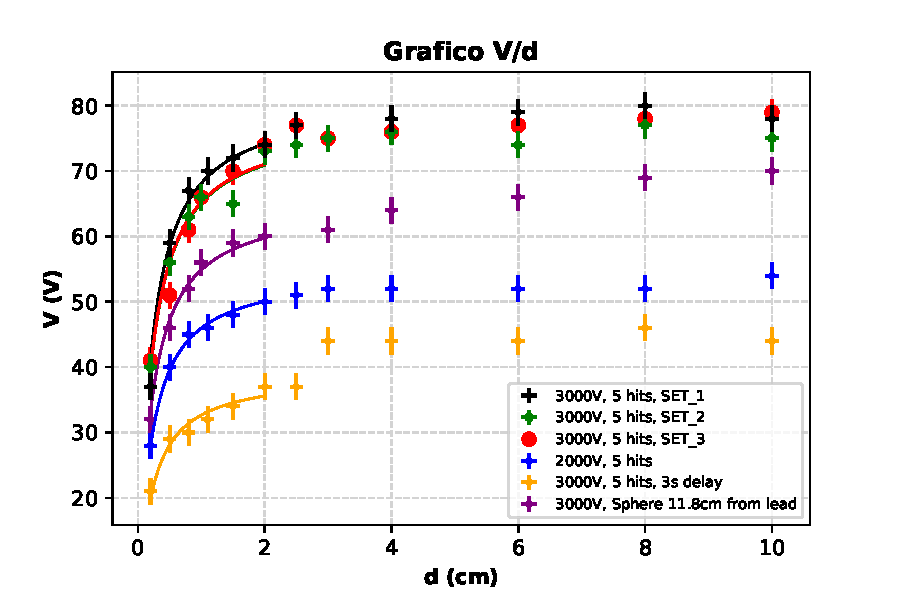
\includegraphics[width=14.5cm]{Figures/Grafico_Parte1.pdf}
  \caption{Grafico della tensione (in Volt) in funzione della distanza (in metri) per sei set differenti. L'errore sulla tensione è pari a $2 V$ mentre quella sulla distanza è di $1 mm$ ovvero il doppio dell'errore di lettura, in quanto presente un errore nella misura della posizione di entrambe le facce del condensatore. Il fit si adatta bene ai dati solo fino a $d = 2 cm$, ovvero in approssimazione $d \ll \sqrt{A} = 15.8 cm$ e non può essere applicato in assenza di questa condizione. Superati i $4cm$ la tensione misurata tende ad un valore di saturazione a causa della capacità del sistema. Si nota inoltre una ripetibilità nei primi 3 set, che sono stati effettuati nelle stesse condizioni.}
  \label{fig:GraficoParteI}
\end{figure}

\begin{figure}[H]
  \centering
  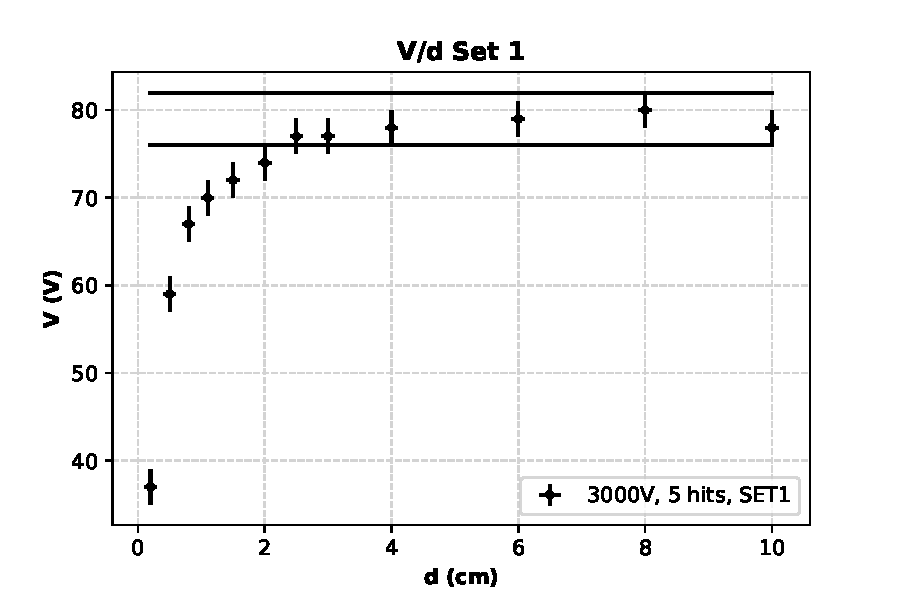
\includegraphics[width=11.5cm]{Figures/Grafico_Parte1_SET1.pdf}
  \caption{Grafico della tensione (in Volt) in funzione della distanza (in metri) per il set 1. Le rette asintotiche sono state tracciate in modo da contenere gli ultimi 3 punti per i quali la capacità del condensatore diventa trascurabile, ponendo quindi in buona approssimazione $V = \dfrac{Q}{C_{sistema}}$}
  \label{fig:parteIset1}
\end{figure}

Per stimare la carica totale $Q$ trasferita al condensatore si considera la sua capacità trascurabile rispetto a $C_{sistema}$ quando la distanza $d \geq 6 cm$, quindi sono state tracciate due rette asintotiche contenenti questi punti come mostrato nel grafico \ref{fig:parteIset1}. Da queste, facendone la semisomma e la semidifferenza si è trovato, per ogni set, il valore di carica presente sul condensatore ed il corrispondente errore.

\begin{align*}
    Q_1 &= (89 \pm 3) 10^{-10} C    &   Q_3 &= (88 \pm 3) 10^{-10} C    &    Q_5 &= (50 \pm 4) 10^{-10} C\\
    Q_2 &= (85 \pm 4) 10^{-10} C    &   Q_4 &= (60 \pm 3) 10^{-10} C    &    Q_6 &= (77 \pm 5) 10^{-10} C
\end{align*}

È stato anche effettuato il calcolo della carica come $Q = (C_{sistema} + C) \cdot V$ per poi fare una media ed una deviazione standard di tutte le misure ottenendo dei valori compatibili con quelli calcolati graficamente.

\begin{align*}
    Q_1 &= (91 \pm 3) 10^{-10} C    &   Q_3 &= (89 \pm 3) 10^{-10} C    &    Q_5 &= (48 \pm 4) 10^{-10} C\\
    Q_2 &= (88 \pm 2) 10^{-10} C    &   Q_4 &= (61.9 \pm 0.9) 10^{-10} C    &    Q_6 &= (75 \pm 3) 10^{-10} C
\end{align*}

Intersecando le barre di errore dei due risultati si sono ottenuti i valori finali di:

\begin{align*}
    Q_1 &= (90 \pm 2) 10^{-10} C    &   Q_3 &= (88.5 \pm 2.5) 10^{-10} C    &    Q_5 &= (49 \pm 3) 10^{-10} C\\
    Q_2 &= (87.5 \pm 1.5) 10^{-10} C    &   Q_4 &= (62 \pm 2) 10^{-10} C    &    Q_6 &= (75 \pm 3) 10^{-10} C
\end{align*}

In particolare la carica presente nei primi 3 set risulta compatibile anche con la carica del quarto set dopo aver moltiplicato il suo valore per $\dfrac{3}{2}$, numero ottenuto dal rapporto delle tensioni a cui era sottoposta la sfera.

\begin{equation*}
    Q_4 \cdot \dfrac{3}{2} = (90 \pm 5) 10^{-10} C 
\end{equation*}

I primi 3 set, ripetuti nelle stesse condizioni, risultano avere una carica compatibile. Intersecando le barre di errore si è quindi ottenuto il risultato finale di:

\begin{equation*}
    Q_{123} = (87.5 \pm 1.5) 10^{-10} C 
\end{equation*}
\par} 
\newpage
\subsection{Risultati Parte II}
{\fontsize{12}{14}\selectfont 

\begin{figure}[H]
  \centering
  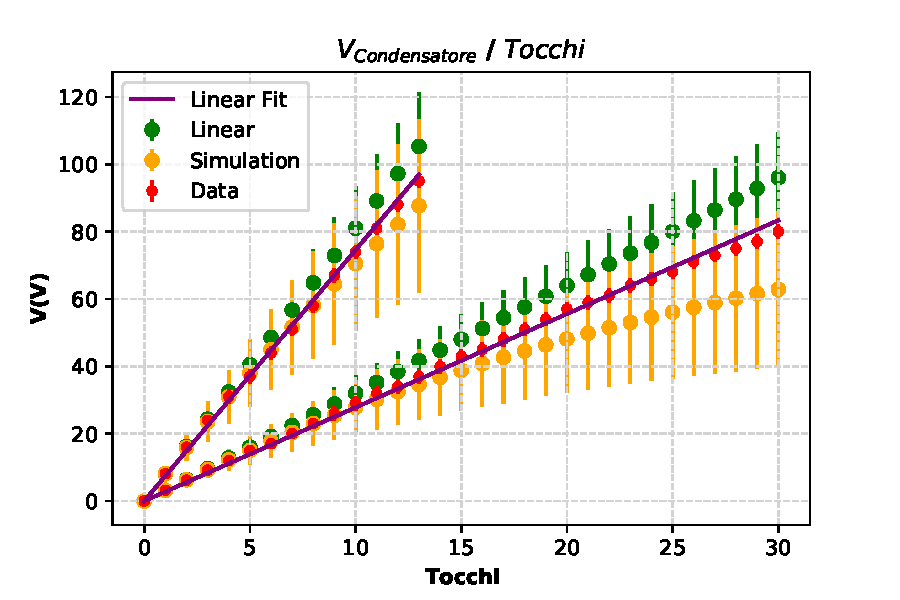
\includegraphics[width=13cm]{Figures/Grafico_Parte2.pdf}
  \caption{Grafico della tensione (in V) in funzione del numero di tocchi per due set differenti. L'errore sulla tensione è pari all'$1\%$ del f.s. + $1$ digit. Le simulazioni si avvicinano all'andamento del rispettivo set di dati ma non lo descrivono esattamente. Il fit è nella forma $V = \text{pendenza} \cdot \text{tocchi}$, quindi passante per lo 0. Nel fit lineare si nota come gli ultimi punti si trovano al di sotto della retta mentre i primi al di sopra di essa, evidenziando come la carica trasferita diminuisca ad ogni tocco.}
  \label{fig:GraficoParteII}
\end{figure}

\begin{figure}[H]
  \centering
  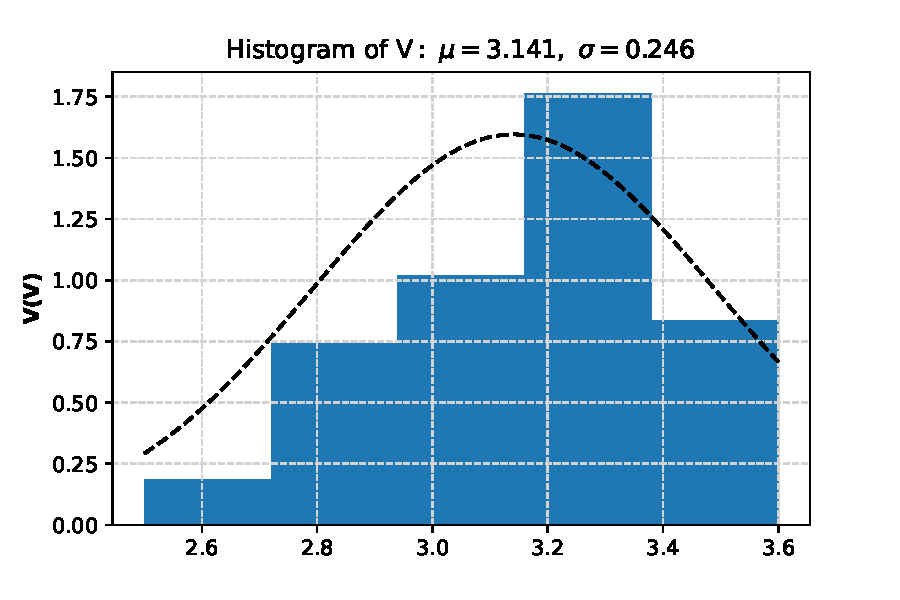
\includegraphics[width=11cm]{Figures/Grafico_Parte2_Carica_Trasferita.pdf}
  \caption{Istogramma della tensione (in V) ai capi del condensatore dopo un tocco, con la sfera carica a $1 kV$. Ci si aspetta una distribuzione gaussiana dei dati che tramite un fit risulta caratterizzata da $\mu = 3.141 V$ e $\sigma = 0.246 V$.}
  \label{fig:GraficoParteIICarica}
\end{figure}

La carica trasferita con il suo errore statistico (ottenuto propagando in quadratura gli errori) è risultata essere:

\begin{equation*}
    Q = \left(C_{sistema} + \dfrac{\varepsilon \cdot A}{d}\right) \cdot V = (4.7 \pm 0.5)\cdot 10^{-10} C
\end{equation*}



\par}

\subsection{Risultati Parte III}
{\fontsize{12}{14}\selectfont 

\begin{figure}[H]
  \centering
  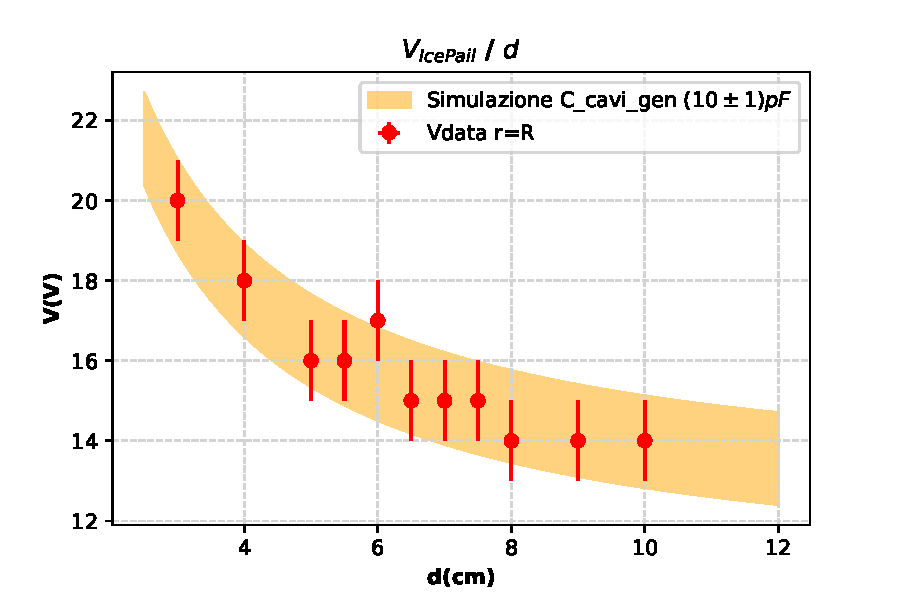
\includegraphics[width=14cm]{Figures/Grafico_Parte3.pdf}
  \caption{Grafico della tensione (in Volt) in funzione della distanza tra le piastre (in centimetri). L'errore sulla tensione è pari a $1.3V$. L'errore sulla distanza è di $1 mm$. La simulazione è stata fatta supponendo una capacità dei cavi che collegano il condensatore al generatore di $(10 \pm 1)pF$, supposizione necessaria ai fini del risultato della simulazione per poter ricreare l'andamento atteso.}
  \label{fig:GraficoParteIII}
\end{figure}


\par} 
\subsection{Risultati Parte IV}
{\fontsize{12}{14}\selectfont 
\begin{figure}[H]
  \centering
  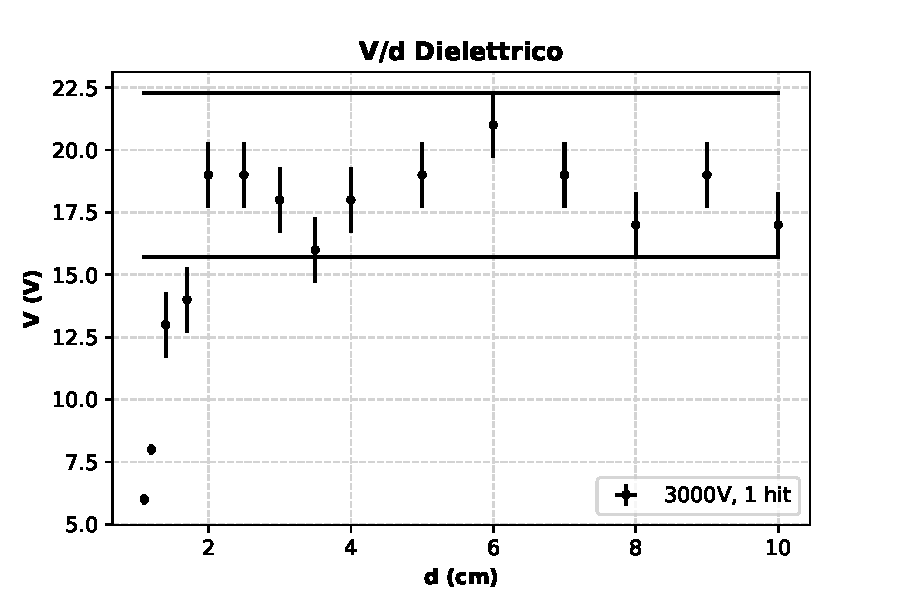
\includegraphics[width=13cm]{Figures/Grafico_Parte4.pdf}
  \caption{Grafico della tensione (in Volt) in funzione della distanza tra le piastre (in cm). L'errore sulla tensione è pari a $1\% $f.s. + $1$ digit, mentre l'errore sulla distanza è di $1 mm$. Sono state tracciate due rette asintotiche nei punti in cui la tensione è arrivata a saturazione. Da queste, facendone la semisomma e la semidifferenza si è trovato il valore di carica presente sul condensatore. La tensione arriva a saturazione dopo una distanza di $2cm$.}
  \label{fig:parteIV}
\end{figure}

Dato che con distanze $d \geq 6cm$ la capacità del condensatore diventa trascurabile rispetto alla capacità del sistema, si considera la tensione $V = \dfrac{Q}{C_{sistema}}$ ottenendo una carica

\begin{align*}
    Q &= (21 \pm 4) 10^{-10} C
\end{align*}

Calcolando invece la carica come $Q = (C_{sistema} + C) \cdot V$ e facendone poi una media pesata ed una deviazione standard si è ottenuto:

\begin{equation*}
    Q = (20 \pm 4)\cdot 10^{-11} C
\end{equation*}

Incrociando le barre di errore dei due set il risultato finale della carica è:
\begin{equation*}
    Q = (20.5 \pm 3.5)\cdot 10^{-11} C
\end{equation*}



\par} 
\section{Conclusioni}
{\fontsize{12}{14}\selectfont 

In questo esperimento è stato possibile studiare un sistema elettrostatico costituito da un condensatore con distanza tra le facce regolabile, esaminando sia il range di distanze in cui vale l'approssimazione di facce piane e parallele, sia per distanze maggiori. 
\par
È stato verificato come la carica si distribuisca sulle piastre del condensatore e che tocchi successivi della \emph{proof plane} trasferiscono meno carica dei precedenti, come atteso dalla teoria.
\par
Per la costruzione dell'istogramma relativo alla carica trasferita da un singolo tocco sarebbe stato opportuno prendere più misure in modo da verificare con una maggiore accuratezza che l'andamento seguisse quello di una gaussiana.
\par
Per alcune parti dell'esperimento sarebbe stato preferibile avere più set di misure per poterne verificare la ripetibilità o per analizzare il comportamento del sistema alla variazione dei parametri al contorno.
\par

Sarebbe stato opportuno adattare il fondoscala dell'elettrometro al valore misurato, accorgimento che non si è sempre riusciti a seguire.
\par}
 

\newpage
\appendix
\renewcommand{\thesection}{\Alph{subsection}}
\renewcommand{\thesubsection}{\Alph{subsection}}
\section*{Appendice}
\addcontentsline{toc}{section}{Appendice}


\subsection{Calcolo Capacità Elettrometro} \label{app:capacitasistema}
{\fontsize{11}{14}\selectfont 

Per stimare la capacità del sistema formato dall'elettrometro più i cavi di connessione, è stato collegato il generatore impostato a $(30.0 \pm 1.5) V$ (per l'errore è stato utilizzato un errore massimo come descritto nel manuale $30V \pm 5\%$) al condensatore con distanza tra le armature $d = (0.3 \pm 0.1) cm$. Una volta caricato il condensatore, il generatore è stato scollegato con l'ausilio di guanti, in modo da evitare dispersione di cariche. 
\par
Per misurare la tensione ai capi del condensatore sono stati attaccati i morsetti dell'elettrometro. La tensione misurata, a parità di carica, è $V_s = (12.0 \pm 1.3) V$.
\par
Infine per il calcolo della capacità e del suo errore massimo è stata usata l'\autoref{eq:capacitasistema} e la relativa propagazione degli errori massimi.

\begin{equation} \label{eq:capacitasistema}
    C_{sistema} = C \cdot \dfrac{V - V_s}{V_s} = (113 \pm 30) pF
\end{equation}


\par
Quindi è stato possibile ricavare la capacità dei cavi ed il corrispondente errore massimo come:

\begin{equation}
    C_{cavi} = C_{sistema} - C_e = (86 \pm 30) pF
\end{equation}
\par}
\subsection{Referenze}
{\fontsize{12}{14}\selectfont 

\begin{itemize}
    \item \href{https://cdn.pasco.com/product_document/Basic-Electrostatics-Sys-Manual-ES-9080B.pdf}{Manuale Pasco}\label{link:pascomanual}
    \item \href{https://github.com/Vayxen/Lab2-Elettrostatica}{Repository GitHub dell'esperimento}
    \item \href{https://github.com/Vayxen/Lab2-Elettrostatica/tree/main/tables}{Tabelle dei dati}
    \item \href{https://github.com/Vayxen/Lab2-Elettrostatica/tree/main/grafici}{Grafici}
\end{itemize}

\par}
\end{document}